\documentclass{cmc}

\usepackage{xcolor}

\begin{document}

\pagestyle{fancy}
\lhead{\textit{\textbf{Computational Motor Control, Spring 2020} \\
    Python exercise, Lab 5, GRADED}} \rhead{Jon Märki, Jérôme Savary, Gabriel Tornare}

\section*{Student names: Jon Märki, Jérôme Savary, Gabriel Tornare}

\section*{Exercise 1 : Hill muscle model}
\label{sec:question-2}

\subsection*{Muscle Force-Length Relationship}
\label{sec:muscle-force-length}

\subsection*{1.a For a given stimulation, explore the relationship
  between active and passive muscle forces and the length of the
  contractile element.  Plot the force-length relationship curve.
  Discuss the different regions in the plot. Use the
  \fileref{isometric\_muscle\_system.py::IsometricMuscleSystem} instance
  to setup your experiment in \fileref{exercise1.py}}

    %%%%%%%%%%%%%%%%%%%%%%%%%%%%%%%%%%%%%%%%%%%%%%%%%%%%%%%%
    %BEGIN USER TEXT%
    %%%%%%%%%%%%%%%%%%%%%%%%%%%%%%%%%%%%%%%%%%%%%%%%%%%%%%%%
    
    The experimentation results are found in Figure \ref{fig:ex_1a}. We decided to modify two parameters:
    \begin{itemize}
        \item muscle\_stretch = 0.5
        \item muscle\_stimulation = 0.7
    \end{itemize}
    
    \begin{figure}[H]
      \centering 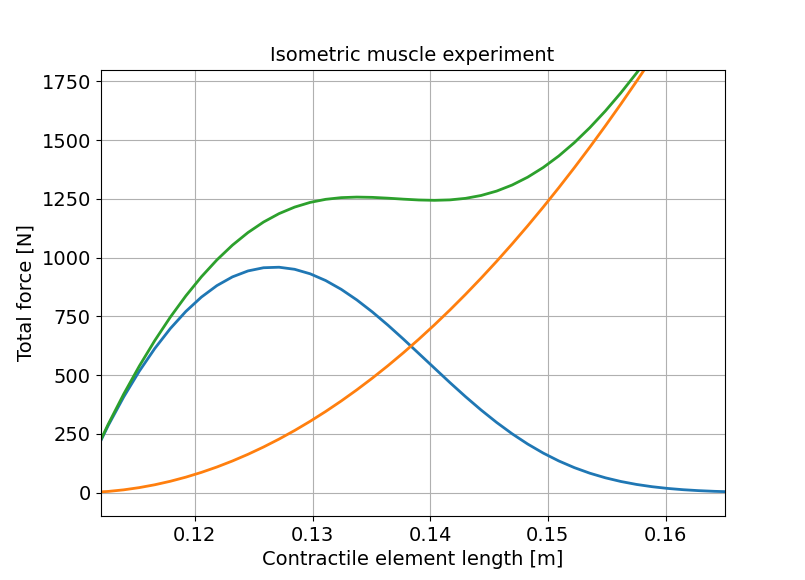
\includegraphics[width=0.7\textwidth]{figures/1a.png}
      \caption{\label{fig:ex_1a} Result of experimentation 1\_a. \textcolor{blue}{Blue: active force [N]}; \textcolor{orange}{Orange: passive force [N]}; \textcolor{green}{Green: total force [N]}}
    \end{figure}
    
    As shown in slide 34 of Lecture 2, the passive force behaviour can be observed when the muscle is stretched from a certain length (when it is not slack anymore) - here this slack region does not exist - due to the spring resistance in the sarcomeres. The harder we pull on the muscle, the stronger the reaction force is, just like a non-linear Hooke law (non-linear spring behaviour), until the sarcomere/fiber/muscle ruptures.
    
    As for the active force, it also depends on the length of the sarcomere, but this time on the overlapping ratio of the actin over the myosin. If the fiber is too contracted, the sarcomere cannot contract that much and does not produce a lot of force. If the fiber is too stretched, there is not enough overlap between the two components to produce a good traction force.
    By adding the two forces together, we can observe that the total force reaches a local maximum (when applying a high enough stimulation, because otherwise we don't have a lot of active force available) at the optimal muscle length, which in our case is 0.13[m].
    
    The total force graph has three main regions:
    \begin{itemize}
        \item From $l_ce$ = 0 to about 0.13[m]: first fast rise of the total force due to predominance of rising active force due to the fact that there is more and more space between the two Z-rings of each sarcomere to allow a good contraction of the myosin relatively to the actin.
        \item from $l_ce$ = 0.13 to about 0.143[m]: plateau of the total force, where the decrease of the active force is compensated by the increase in the passive force.
        (the negative effect of the decreasing overlap actin-myosin on the active force overtook the positive effect of the space increase between the Z-rings since before we reached the optimal length).
        \item from $l_ce$ = 0.143 to the muscle rupture: new rise of the total force, for the increase of the non-linear spring-reactive passive force is bigger than the decrease of the active force.
    \end{itemize}
    
    %%%%%%%%%%%%%%%%%%%%%%%%%%%%%%%%%%%%%%%%%%%%%%%%%%%%%%%%
    %END USER TEXT%
    %%%%%%%%%%%%%%%%%%%%%%%%%%%%%%%%%%%%%%%%%%%%%%%%%%%%%%%%

\subsection*{1.b In (1.a), you explored the muscle force-length
  relationship for a given stimulation. What happens to the
  relationship when the stimulation is varied between [0 - 1]? Support
  your response with one plot showing the different force-length
  relationship curves.}

    %%%%%%%%%%%%%%%%%%%%%%%%%%%%%%%%%%%%%%%%%%%%%%%%%%%%%%%%
    %BEGIN USER TEXT%
    %%%%%%%%%%%%%%%%%%%%%%%%%%%%%%%%%%%%%%%%%%%%%%%%%%%%%%%%
The measurements on different stimulation values can be found on Figure \ref{fig:ex_1b}.

    \begin{figure}[H]
      \centering 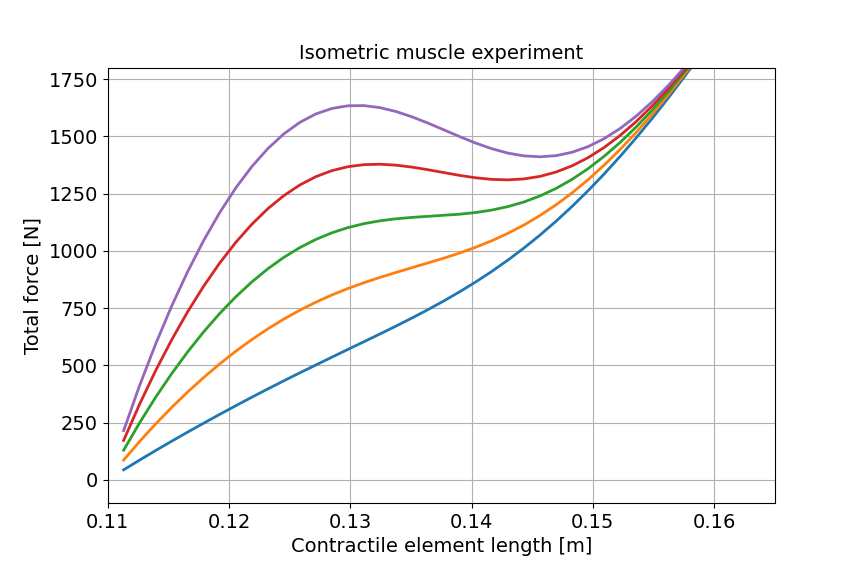
\includegraphics[width=0.7\textwidth]{figures/1b stim.png}
      \caption{\label{fig:ex_1b} Result of experimentation 1\_b. \textcolor{blue}{stimulation = 0.2[N]}; \textcolor{orange}{stimulation = 0.4[N]}; \textcolor{green}{stimulation = 0.6[N]}; \textcolor{red}{stimulation = 0.8[N]}; \textcolor{violet}{stimulation = 1[N]}}
    \end{figure}
    
    As explained in part 1.a, a lower stimulation implies that the active force will be lower at the same muscle length, which means that the predominant force will be the passive one.
    %%%%%%%%%%%%%%%%%%%%%%%%%%%%%%%%%%%%%%%%%%%%%%%%%%%%%%%%
    %END USER TEXT%
    %%%%%%%%%%%%%%%%%%%%%%%%%%%%%%%%%%%%%%%%%%%%%%%%%%%%%%%%

\subsection*{1.c Describe how the[N] fiber length ($l_{opt}$) influences
  the force-length curve.  (Compare a muscle comprised of short muscle
  fibers to a muscle comprised on long muscle fibers.). To change the
  parameter you can use
  \fileref{system\_parameters.py::MuscleParameters} before
  instantiating the muscle. No more than two plots are required. }

    %%%%%%%%%%%%%%%%%%%%%%%%%%%%%%%%%%%%%%%%%%%%%%%%%%%%%%%%
    %BEGIN USER TEXT%
    %%%%%%%%%%%%%%%%%%%%%%%%%%%%%%%%%%%%%%%%%%%%%%%%%%%%%%%%
    
    The result of the exercise 1.c can be found on Figure \ref{fig:ex_1c}.
    
    \begin{figure}[H]
      \centering 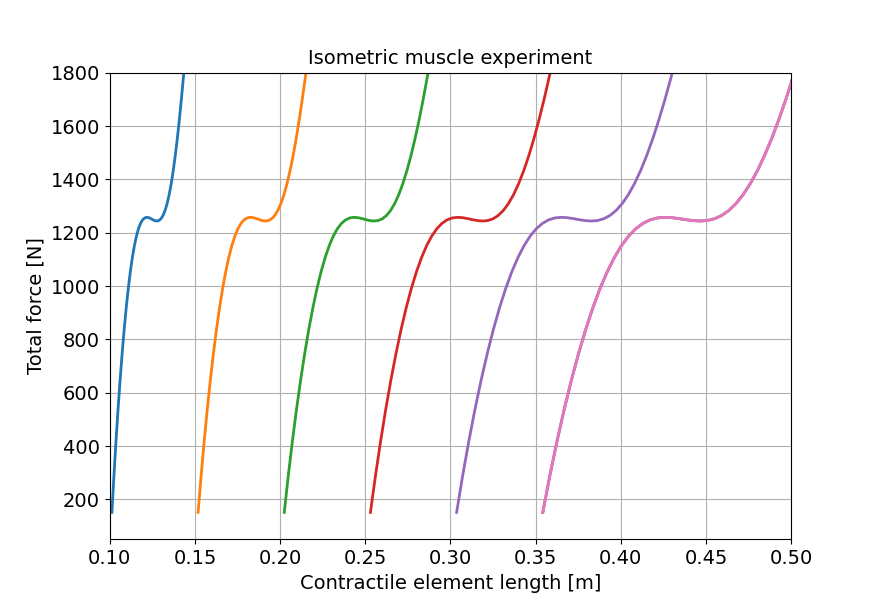
\includegraphics[width=0.7\textwidth]{figures/1c.png}
      \caption{\label{fig:ex_1c} Result of experimentation 1\_c: L\_opt =:  \textcolor{blue}{ 0.10[m]}; \textcolor{orange}{ 0.15[m]}; \textcolor{green}{ 0.2[m]}; \textcolor{red}{ 0.25[m]}; \textcolor{violet}{ 0.3[m]}; \textcolor{pink}{ 0.35[m]} }
    \end{figure}

    We can observe that a longer muscle fiber has a bigger plateau near the optimal fiber length, which is in turn further away from the initial fiber length than for a shorter muscle fiber. This can be explained by the fact that the active force will decrease less rapidly because the myosin and actin will be overlaped for a longer period of time after exceeding the optimal length.
    %%%%%%%%%%%%%%%%%%%%%%%%%%%%%%%%%%%%%%%%%%%%%%%%%%%%%%%%
    %BEGIN USER TEXT%
    %%%%%%%%%%%%%%%%%%%%%%%%%%%%%%%%%%%%%%%%%%%%%%%%%%%%%%%%

\subsection*{Muscle Velocity-Tension Relationship}
In this exercise you will explore the relation between the force and
velocity of the muscle. In order to do this we replicate the set-up
shown before.%Attention ici - ?? Here the length of the muscle
is allowed to vary by attaching one of its end to a fixed point and
the other to a variable external load. While applying a constant load
initially and holding the muscle at constant length, a quick release
is performed to let the muscle contract and pull the weight. The
maximum velocity during this quick release will give us the
relationship between muscle contractile velocity and the force.


\corr{Note} : Since the velocity changes sign and you need to compute the maximum
velocity accordingly by checking if the muscle was stretched or compressed
at the end of the experiment.

\begin{equation}
  \label{eq:2}
 V_{ce} = \left\{
\begin{array}{ll}
      max(v_{ce}(t)) & l_{mtu} < (l_{opt} + l_{slack}) \\
      min(v_{ce}(t)) & else \\
\end{array}
\right.
\end{equation}

\subsection*{1.d For a stimulation of 1.0 and starting at optimal
  muscle length, explore the relationship between contractile element
  velocity and external load. Plot the Velocity-Tension relationship
  curve. Include shortening and lengthening regions. Use the
  \fileref{isotonic\_muscle\_system.py::IsotonicMuscleSystem} instance
  to setup your experiment in \fileref{exercise1.py}}
  
    %%%%%%%%%%%%%%%%%%%%%%%%%%%%%%%%%%%%%%%%%%%%%%%%%%%%%%%%
    %BEGIN USER TEXT%
    %%%%%%%%%%%%%%%%%%%%%%%%%%%%%%%%%%%%%%%%%%%%%%%%%%%%%%%%
    The result of the exercise 1.d can be found on Figure \ref{fig:ex_1d}.
    
    \begin{figure}[H]
      \centering 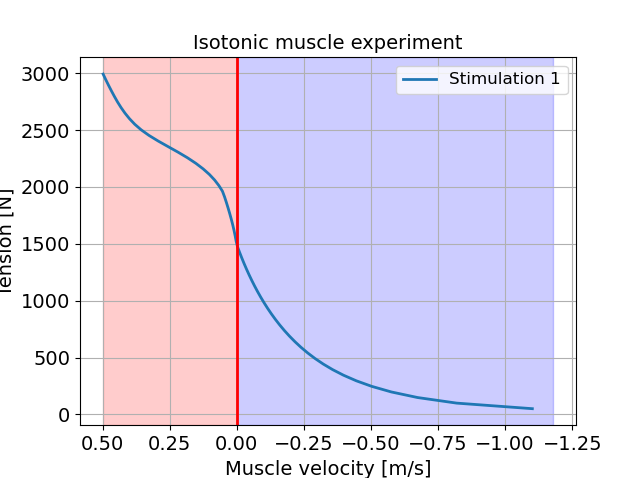
\includegraphics[width=0.7\textwidth]{figures/1d.png}
      \caption{\label{fig:ex_1d} Result of experimentation 1\_d. In red: lengthening region, in blue: shortening region}
    \end{figure}
    
    %%%%%%%%%%%%%%%%%%%%%%%%%%%%%%%%%%%%%%%%%%%%%%%%%%%%%%%%
    %BEGIN USER TEXT%
    %%%%%%%%%%%%%%%%%%%%%%%%%%%%%%%%%%%%%%%%%%%%%%%%%%%%%%%%

\subsection*{1.e For the muscle force-velocity relationship, why is
  the lengthening force greater than the force output during
  shortening? No plots necessary}

    As explained graphically in slide 35 of the lecture 5, when the muscle is being lengthened, we are working against the actin-myosin interaction direction, which means that we need a higher force to obtain the same deformation velocity than in the shortening direction.

\subsection*{1.f What happens to the force-velocity relationship
  when the stimulation is varied between [0 - 1]? Support your
  response with one plot showing the different force-velocity
  relationship curves.  }
  
    %%%%%%%%%%%%%%%%%%%%%%%%%%%%%%%%%%%%%%%%%%%%%%%%%%%%%%%%
    %BEGIN USER TEXT%
    %%%%%%%%%%%%%%%%%%%%%%%%%%%%%%%%%%%%%%%%%%%%%%%%%%%%%%%%
    
    The result of the exercise 1\_f can be found on Figure \ref{fig:ex_1f}.
    
    \begin{figure}[H]
      \centering 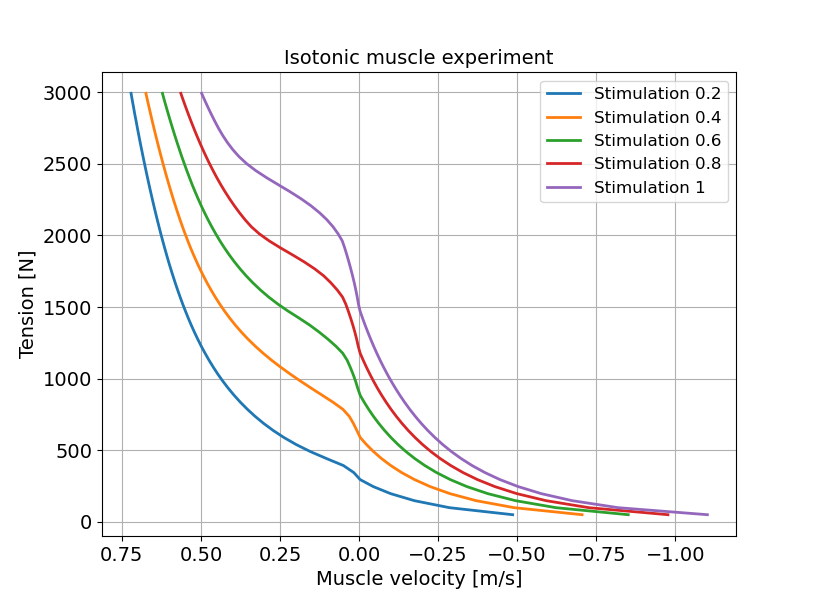
\includegraphics[width=0.7\textwidth]{figures/1f.png}
      \caption{\label{fig:ex_1f} Result of experimentation 1\_f}
    \end{figure}
    
    A more stimulated muscle fibre needs more force to be lengthened and shortened because the actin-myosin interaction will be stronger, therefore harder to act upon.
    
    %%%%%%%%%%%%%%%%%%%%%%%%%%%%%%%%%%%%%%%%%%%%%%%%%%%%%%%%
    %BEGIN USER TEXT%
    %%%%%%%%%%%%%%%%%%%%%%%%%%%%%%%%%%%%%%%%%%%%%%%%%%%%%%%%  

\end{document}
